\chapter{General Scientific Introduction}
\selectlanguage{english}

\begin{flushright}
    \textit{''A major challenge of any scientific endeavor is not only to provide good answers to the questions we ask about our world, but to find good questions to ask in the first place.''}\\
    Paul Cisek, Resynthesizing behavior through phylogenetic refinement, 2019
\end{flushright}

\chaptertoc{}


 
\section{The problem under study}
An introduction to a complex problem is arguably simplified by the use of a well-defined general theory. Alas, while neuroscience lacks something similar to physics' standard model \cite{cottingham2023introduction}, it has a rich history of integrative frameworks designed for a particular sub-fields of investigations. David Marr's three levels of analysis, originally developed to understand vision\cite{marr1982vision}, is one such integrative framework, that has since then been successfully applied to numerous other problems\cite{mcclamrock1991marr,peebles2015thirty}. To understand the complex "problem of vision", Marr proposed three levels of approach: the computational level (examining the system's purpose), the algorithmic level (exploring its procedural mechanism), and the implementational level (detailing practical aspects). Our present introduction adheres to this logical structure.

The general aim of this manuscript is to understand the purpose of variance-related computation in the brain (computational level), the logic behind such computations (algorithmic level), and the methods to enable both brains and machines to perform these computations (implementational level). 
As we shall see in the following sections, our approach will naturally lean towards Bayesian inference as a framework to articulate the problem(s) of vision. Bayesian schemes, like related probabilistic methods~\cite{aitchison2017or}, are extremely valuable in making predictions about experimental outcomes, but are not designed to provide mechanistic explanations for those outcomes. In that sense, the descriptive models used in this thesis work synergistically well with Marr's approach \cite{colombo2012bayes} for one key reason: the \textit{formal independence} of the three levels. Practically, this means that different algorithms can be used to solve the same computational problem, and that different hardware (or biological substrates) can implement the same algorithms. Therefore, computational level questions are \textit{formally independent} from other levels, allowing them to be addressed without constraints from other levels. 
It then becomes that the relationship between the three levels is one of \textit{realization}, that is, of incremental assembly. In the specific case of variance computations, this will allow us to start focusing on the "what" without being preoccupied with the "why", and then similarly with the "how", thus building this introduction incrementally from the descriptive to the explanatory.



\newpage



\subsection{The computational level: Vision in an uncertain world}
Marr's first level of analysis, the computational level, seeks to describe the purpose of the system under study. Rather than deriving a working theory from the data, this allows us to approach the theory first, then work our way towards facts progressively. This section of the introduction is thus concerned with the idea of framing vision as an uncertain process.

However, as with all theses that relate to a particular sensory system, we cannot escape the required description of the system under scrutiny, which is here the neurobiology of visual processing. While this arguably pertains more to the implementational aspect of Marr's three levels, and thus should be discussed last, starting by introducing the notion of "orientation selectivity" in \gls{V1} considerably simplifies the remainder of the introduction. Overall, we aim to be rather synthetic here, quickly working our way from the retina towards \gls{V1}. 

We then dive properly into the computational nature of the inputs to the visual system, be they natural or synthetic, with a focus on the sources of uncertainty in vision. Finally, we discuss probabilistic accounts of vision and their (numerous) successes, which will serve as a justification of the algorithmic approach, described in the Section 2.1.2.



\subsubsection{The neurobiology of vision \textit{ante} V1}
With a few niche exceptions, vision is a sense present ubiquitously throughout in the animal domain~\cite{land2018eyes}. Vision is nothing short of a marvel of biology, a sense that starts by capturing massless elements of electromagnetic radiations, the photons, eventually converting them into a coherent representation of our environment. The general computational goal of vision is conserved throughout various species, but its implementation varies extraordinarily: sixty pair of eyes in scallops~\cite{palmer2017image}, polarized facets optimized for tracking mating partners in horseflies~\cite{horvath2017horseflies}, hyperspectral cameras in mantis shrimps~\cite{thoen2014different}, several segregated nervous ganglia for visual processes in octopuses~\cite{young1962optic}... In the case of primates, our specific tweaking of vision is the dedication of almost a third of our cortex to processing visual inputs~\cite{kandel2000principles}. As fascinating as shrimp vision might be, we will here focus on a human-centric account of vision, namely describing of the primate visual system (Figure \ref{fig_chap2_vision_overview}). However, given that chapters 4 and 7 deal with neural data acquired from anesthetized cats, we will finish this section with a brief comparison of the two species, as animal models used commonly in visual neuroscience. 

\begin{figure}[h!tbp]
\vspace{0.5cm}
\centering
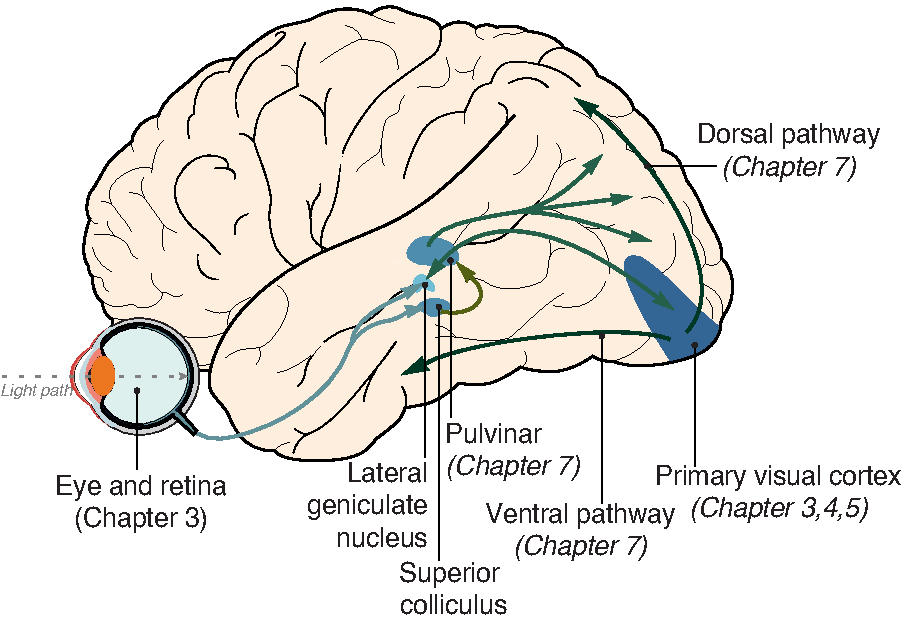
\includegraphics[width=.9\textwidth]{fig/chap2_fig_visual_system.pdf}
\caption[A schematic overview of the visual system.]{A schematic overview of the visual system. Electromagnetic waves (photons) are transduced in the retina into binary neural activity (spikes), which are then transmitted through the optic nerve to the \gls{LGN}, and then to \gls{V1}, before being processed by further cortical areas. The present chapter introduces general notions to the visual system, with specific part discussed further in the chapters indicated here in \textit{italics}. Figure adapted from~\cite{kandel2000principles}.}
\label{fig_chap2_vision_overview}
\end{figure}

Vision relies on a sophisticated bilateral sensing organ, the eye, which can be likened to an extraordinarily intricate adjustable-focus camera (Figure \ref{fig_chap2_vision_eye_retina}). Light enters the eye via the cornea, continues through the transparent aqueous humor, and proceeds through the pupil, which the opening of an aperture-regulating diaphragm, the iris. The focusing of the light source is then performed by the biconvex lens of the crystalline, which is dynamically adjusted by tiny muscles that modify the focal length. The nervous system thus possesses control over these components, enabling visual signals to act as feedback for adjusting the eye's optical characteristics in a closed-loop system~\cite{fernandez2001closed}.

\begin{figure}[h!tbp]
\vspace{0.5cm}
\centering
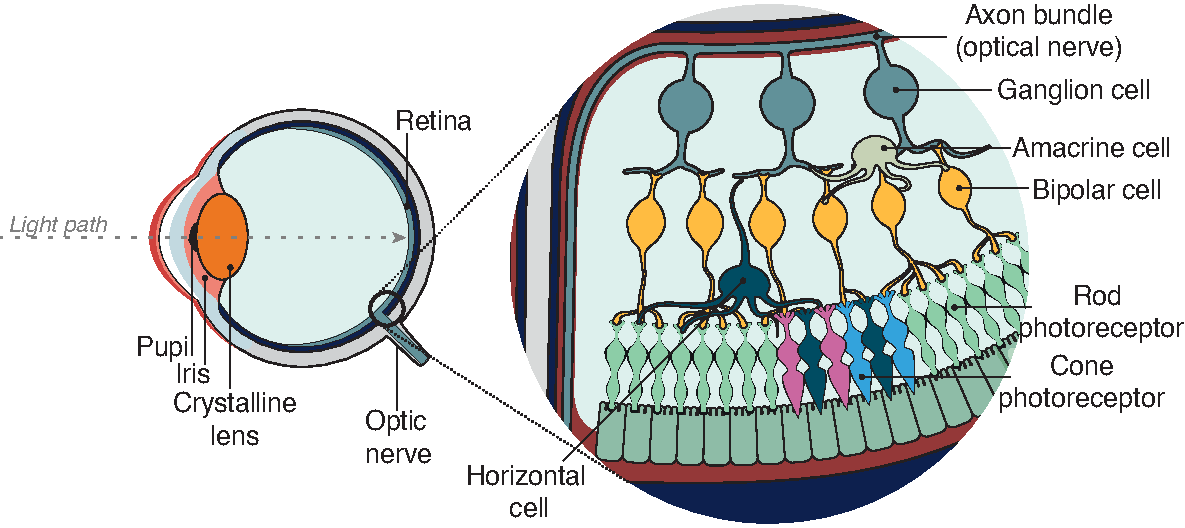
\includegraphics[width=.9\textwidth]{fig/chap2_fig_retina.pdf}
\caption[Illustration of the eye and retina.]{Illustration of the eye and retina. Adapted from~\cite{holmes2018reconstructing}.}
\label{fig_chap2_vision_eye_retina}
\end{figure}
Only then does light reach the photosensitive surface situated at the rear of the eye: the retina. Interestingly, the light must also traverse the full depth of the retina before being actually captured, as the light-sensitive part of the retina lies in its depth rather than on its surface. This propagation through the retina disperses the light, resulting in a somewhat lower-quality image. However, this is compensated for by a particular type of cell that channels light~\cite{newman1996muller}, but also contributes to a space-efficient design~\cite{kroger2009space}. 
A unique feature resulting from this architecture is that the axons from the retina's neurons must exit through the posterior section of the eye, and in doing so, must traverse the retinal depth in its entirety in some place. This is done in a single location, known as a "scotoma", which is thus devoid of photoreceptors and lacks direct visual input. However, this visual gap is seamlessly filled in, rendering it unnoticed in our conscious experience~\cite{rohrschneider2004determination}.

Aside to this particular design, the retina is a remarkably effective sensor. Specialized cells, the photoreceptors, convert light into electrical signals via a photosensitive molecule named retinal. These photoreceptors cells come in two varieties: cones, which cover different portions of the visible spectrum, providing important color visual information that we shall not be concerned with in this thesis~\cite{gegenfurtner2003color}; and rods, which are useful in situations with low light intensity. These photoreceptors are distributed in a particular pattern throughout the retina, where the densest concentration of cones is found near the center of the visual field, in the "fovea". This means that in order to obtain the maximum density of light-sensing cells, and thus extract the maximum amount of visual information, the eye must hover in to points of interests~\cite{friston2012perceptions}, which occurs about every hundred of milliseconds in primates~\cite{ibbotson2011visual}. 

The signals from these two types of cells are conveyed in a two-stream parallel process: either to the bipolar cells, carrying feedforward signal processing~\cite{ghosh2004types}, or to the horizontal cells, which carry out lateral integration in the retina, a process that contributes to enhancements in contrast~\cite{masland2012neuronal} and the early recognition of motion~\cite{olveczky2003segregation, liu2021predictive}. The output of this whole early sensory processing is carried out by retinal ganglion cells, whose axons are bundled into the optic nerve and sent deeper into the brain.

This nerve eventually reaches the brain's central hub, the thalamus. In the particular case of the optic nerve, the dedicated thalamus nucleus that receives inputs from the optic nerve is the \gls{LGN}, which is located in the posterior part of the thalamus. The wiring from the retina to the \gls{LGN} is not straightforward, in the literal sense, as part of both eyes' field of view will cross each other over before reaching the thalamus, likely due to an evolutionary twist of the body plan that also resulted in similar decussation (crossing of the middle plane) in the spine~~\cite{kinsbourne2013somatic, larsson2013optic}.
To simply label the thalamus as a relay would be a major oversimplification~\cite{sherman2007thalamus}, as the inputs from the retina to the thalamus represent less than one tenth of the synapses~\cite{ghodrati2017towards}, which might translate into even less than one tenth of actual functional impact~\cite{briggs2011corticogeniculate}.

%Different types of retinal ganglion cells are partitioned into layers within the thalamus of primates, including humans, several types of \gls{LGN} cells convey different kinds of visual information: P cells (Parvocellular), M cells (Magnocellular), and K cells (Koniocellular). P cells are relatively small, and convey information about fine details and color ; M cells are relatively large and convey information about motion and rapid temporal changes ; K cells are less understood, but seem to be linked in the integration of visual and non-visual information~\cite{kaplan2004m}. 

\begin{figure}[h!tbp]
\vspace{0.5cm}
\centering
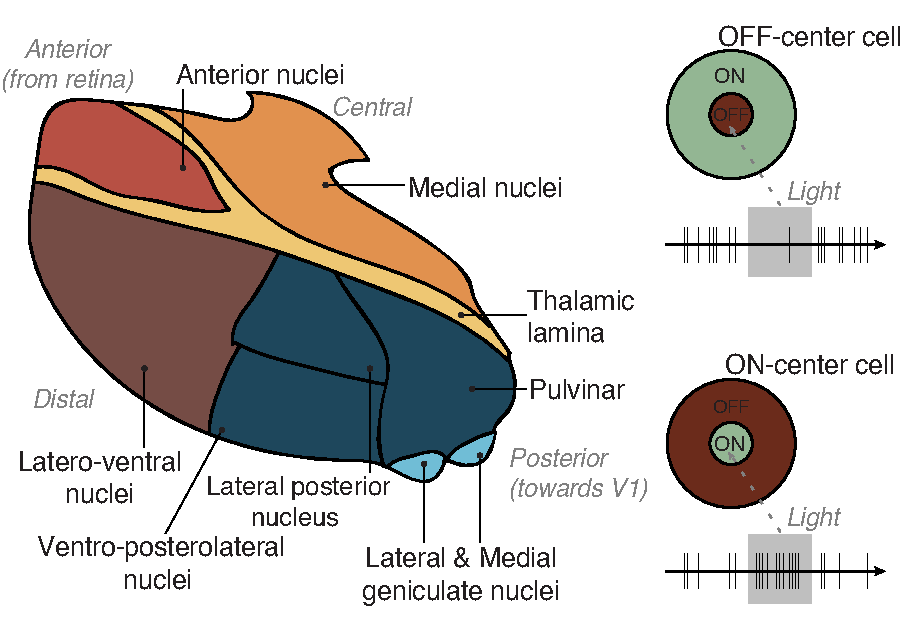
\includegraphics[width=.9\textwidth]{fig/chap2_fig_lgn.pdf}
\caption[Illustration of the \gls{LGN} and nearby thalamic nuclei.]{(left) Anatomy of the \gls{LGN} and nearby thalamic nuclei. Afferences from the optic nerve arrive at the \gls{LGN}. The superior colliculus, located near the cerebellum, is not represented. (right) Illustration of the ON/OFF activation of neurons in the \gls{LGN}.}
\label{fig_chap2_vision_lgn}
\end{figure}

Effectively, the \gls{LGN} acts as the preliminary stage for information consolidation, characterized by cells that perform an ON/OFF transformation of visual input, inherited from the mode of action of retinal ganglion cells (Figure \ref{fig_chap2_vision_lgn}). ON-center cells are triggered by an increase in light intensity within the central portion of their responsive visual field, known as the "receptive field". Conversely, they are deactivated by an increase in light intensity at the periphery of their receptive field. OFF-center cells function in the opposite manner. This shift signifies the transition from encoding unipolar light intensity in the early retina to bipolar light intensity in the thalamus, a crucial transformation for encoding contrast, which paves the way for encoding complex features in the cortex. 

Throughout this thesis, this notion of "receptive fields" (mostly in \gls{V1}) will be central to the subject of study. It is thus worth to define it clearly here, and for that, we will follow its textbook definition as the region in the sensory space in which a stimulus modulates the activity of a neuron. For Sir Charles Sherrington, who coined this term, a receptive field was exemplified by the skin area that, when stimulated, modulated the activity of scratch reflex neurons in canines~\cite{sherrington1906observations}. In our context, a receptive field will always pertain to the spatial configuration of a visual stimulus that modulates the activity of a given neuron in \gls{V1}.

Before we progress to our ultimate stop, \gls{V1}, it's important to recognize the existence of what are referred to as "non-canonical" pathways from the retina. The superior colliculus, for example, constitutes about $10\%$ of the visual output of the retina in primates, though this proportion is increased to $50\%$ for the cat~\cite{orban2012neuronal}. Similarly, the pulvinar nucleus of the thalamus, while only briefly mentioned here, warrants major discussion in the introduction to chapter 7, as it plays an integrative role among various cortical areas while also integrating inputs from the retina~\cite{casanova2004functions}.  



\subsubsection{The neurobiology of vision \textit{intra} V1}
Following this five-page overview of precortical vision stages, we now shift our focus to the primary subject of this thesis: the primary visual cortex, \gls{V1}. Located in the most posterior region of the brain, the occipital lobe, it is also known as the striate cortex, due to the presence of the line of Gennari~\cite{glickstein1984francesco}, a massive bundle of axons originating from the \gls{LGN} that forms a stripe that can be observed with the naked eye.

\begin{figure}[h!tbp]
\vspace{0.5cm}
\centering
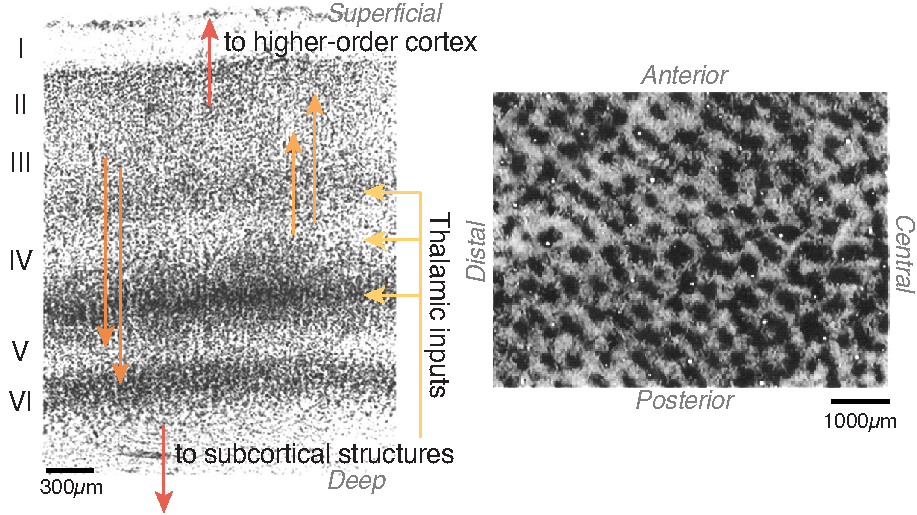
\includegraphics[width=.9\textwidth]{fig/chap2_fig_V1.pdf}
\caption[Primary visual cortex's anatomy.]{Primary visual cortex anatomy. (left) Nissl staining showing the vertical organization of macaque \gls{V1}, adapted from~\cite{schmolesky2011primary}. (right) Cytochrome oxydase staining, reflecting the horizontal organization of the thalamic inputs~\cite{takahata2016does}, adapted from~\cite{murphy1998spacing}.}
\label{fig_chap2_vision_V1}
\end{figure}

In terms of anatomy, like all non-motor cortices~\cite{shipp2013reflections}, \gls{V1} is composed of six layers. Despite ongoing debates surrounding the concept~\cite{horton2005cortical}, the "canonical" circuitry of this layered cortex suggests that visual information enters from the \gls{LGN} into the IVth cortical layer, is transported to layers II and III, and subsequently reaches layers V and VI~\cite{binzegger2004quantitative,douglas2004neuronal}. As we will see later in this introduction, this seemingly simplistic anatomical description is highly beneficial, as this pattern of connectivity is replicated across the whole cortex and can be thus mapped to general computations~\cite{douglas1989canonical, bastos2012canonical}. Organized orthogonally with respect to the cortical surface, this pattern establishes what is often referred to as a "cortical microcolumn.". Depending on the anatomist and the definition, its diameter fluctuates between 200 and 800 µm~\cite{mountcastle1997columnar}. Beyond this local anatomy, one should also note that layers II and III extend sizeable "lateral" axons, forming a "horizontal" circuitry~\cite{angelucci2006contribution,chavane2011lateral} that interconnects multiple similar microcolumns.

One can then naturally inquire about the functionality of these aforementioned circuit motifs. The main functional description of \gls{V1} can be traced back to a seminal study by Hubel and Wiesel, who conducted recordings from individual neurons in this area and discovered neural responses elicited for light bar of specific orientation~\cite{hubel1959receptive, hubel1962receptive}. Functionally, this feature expands upon the ON/OFF structure found in the \gls{LGN}, but incorporates a spatial layout that is lengthened, and thus appropriate for detecting edges in the visual field. Two distinct classes of cells demonstrate this "orientation selectivity": simple and complex cells. Simple cells, aptly named, react to edges of various orientations, and can be thought of as the convergence of many \gls{LGN} cells. Complex cells, on the other hand, exhibit overlapping ON and OFF fields and some degree of spatial invariance, and can be conceptually understood as a hierarchical~\cite{hubel1962receptive} (or lateral~\cite{chance1999complex}) convergence of several simple cells~\cite{boutin2022pooling}. Coherently, the majority of simple cells are found in layer IV and VI, whilst complex cells tend to be confined to layers II and III~\cite{payne2001cat}.
At the broader (mesoscale) level, the selectivity to orientation is arranged into maps of preferred orientation~\cite{grinvald1986functional}, where adjacent cells encode different orientations. This arrangement can be seen as essentially a competition for the best representation of objects that are present at a specific point within the visual field~\cite{kastner2001neural}. For a further detailed account of orientation selectivity, we refer the reader to chapter 4's introduction.

\begin{figure}[h!tbp]
\vspace{0.5cm}
\centering
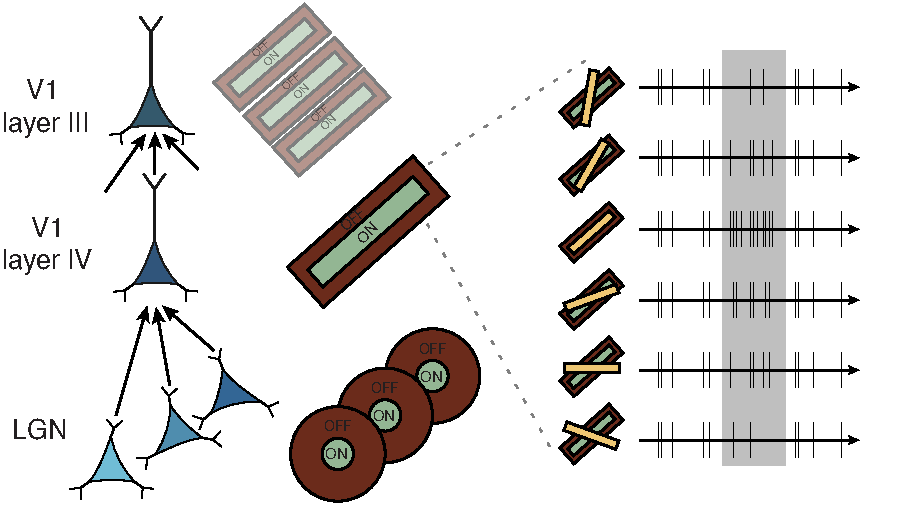
\includegraphics[width=.9\textwidth]{fig/chap2_fig_V1_ori_selec.pdf}
\caption[Illustration of orientation selectivity in V1.]{Illustration of orientation selectivity in \gls{V1}, as a hierarchical model~\cite{hubel1962receptive} from unoriented \gls{LGN} neurons, to simple then complex \gls{V1} cells.}
\label{fig_chap2_vision_V1_ori_selec}
\end{figure}

While orientation selectivity is the core concern of this thesis, there exists also other visual properties encoded by \gls{V1}. A non-exhaustive list would contain the spatial frequency~\cite{tolhurst1981variety}, referring to the scale of a specific feature and to its repeated size in the visual field. Like orientation, spatial frequency is also represented in a spatial frequency map that seems to be independent of orientation selective maps~\cite{issa2000spatial}. Possibly the most critical visual property encoded by \gls{V1} asides orientation is visual eccentricity and elevation, i.e. the spatial localization of visual stimuli~\cite{wandell2007visual}. In primates, there is a specific and highly ordered mapping of the visual field onto the topology of \gls{V1} that is well-captured by a mathematical "log-polar" transformation~\cite{traver2010review}. The closer a particular region of \gls{V1} is to the midline border, the more centrally located within the fovea that region's corresponding visual field will be. This precise arrangement allows for the efficient processing of visual information, enabling dense dedicated regions in the retina to have similar dense dedicated processing region in \gls{V1}. This density spreads throughout the cortical area, thereby providing an "over-representation" of the central portion of the visual field (encoded by the foveal region), with respect to its peripheral portions~\cite{jeremie2023retinotopy}.

V1 is not solely influenced by feedforward and local lateral interactions. It is, in fact, an integral component of a meticulously organized hierarchical network~\cite{scannell1995analysis}. \gls{V1} extends projections to various "extrastriate" cortical areas, such as V2, V4, and IT, as well as to subcortical areas, such as the pulvinar. While the role of these pathways will be occasionally referenced throughout the articles compiled in this thesis, they are not a primary focus of ours, and will be thus reserved for their respective dedicated chapters (4 and 7).

As these chapters also deal with neural recordings gathered from anesthetized cats, one should note a few differences between theirs and the primates' visual systems.
While both possess a primary visual cortex, or \gls{V1}, primates have a greater number of color-detecting cones leading to better color perception, whereas cats have more rods~\cite{sterling1983microcircuitry, kolb1984neural} aiding their low-light vision and 3D motion estimations, due to their nocturnal niche. \\
The main difference that concerns us however lies in \gls{V1}. At the macroscale, the cat's \gls{V1} is composed of Broadmann areas 17 and 18, instead of a single area in primate. Area 17, which was the targeted recording region in chapter 4, receives signals from the cat's equivalent of primate \gls{LGN}'s P cells (X in cats, concerned with fine details) and M cells (Y in cat, concerned with motion information)~\cite{stone1973projection}. Area 18 on the other hand mainly receives axons from the Y cells~\cite{payne2001cat}. 
At the mesoscale, likely to their respective cortical sizes and number of neurons~\cite{kaschube2014neural}, the cortical maps in \gls{V1} have different shapes~\cite{schmidt2021punctuated}, but both species show columnar organization, unlike rodents~\cite{kaas2022escaping}. 
At the microscale, it seems that the general pattern of connectivity is similar, but with difference in specificities of laminar connections, namely from layer IV to III~\cite{lund1979anatomical}. 
The reason for this seemingly mixed model usage in the literature is partly accounted by the fact that cats have been the main historical model under study. As such, the wealth of 60 years of data gathered in the cat visual system, combined with the complexity involved in primate experiments, still makes them highly relevant to vision research. 



\subsubsection{The statistics of natural and naturalistic visual inputs}
Having introduced the basic notions of orientation selectivity and the neurobiological substrates of vision, we can now turn back to the goal we had set in the first place: provide a computational account of vision.

Understanding what vision does, without understanding what type of input vision must process, would be a daunting task. Vision is tasked with processing the complexity and richness of the images that form our everyday perceptual experiences, colloquially known as "natural images". These images, despite their immense diversity and complexity, are all governed by the same physical laws~\cite{stevens1974patterns}, leading to observable statistical regularities. This proves to be an essential feature, given that the neural activity required to process these images is energetically costly~\cite{laughlin1998metabolic}. Further, any sensory processing is under the constraint of extreme time efficiency required for the survival of our organisms~\cite{thorpe1996speed, kirchner2006ultra}.
Horace Barlow~\cite{barlow1961possible} posited that up to \gls{V1}, the purpose of vision is to eliminate such statistically redundant data, thereby optimizing energy usage and speeding up computations. This perspective, often referred to as efficient coding~\cite{olshausen1996natural} allows providing a quantitative description of sensory systems with respect to their environments~\cite{simoncelli2001natural}.

\begin{figure}[h!tbp]
\vspace{0.25cm}
\centering
\includegraphics[width=.9\textwidth]{fig/chap2_fig_natimg.pdf}
\caption[An example of natural image statistics.]{(top) An example of natural image, Marseille's "calanques"~\cite{ladret2023cortical}, with local distribution of orientations shown on the right for multiple patches. (bottom) The statistics of this image, from left to right: distribution of luminance, cumulative luminance frequency, $1/f^2$ Fourier power spectrum.}
\label{fig_chap2_stats_natimg}
\end{figure}

We will here overview such quantitative accounts to get a better sense of the structure of the visual world. Such structure will eventually lead us to a formulation of vision as a variance-bound problem. Fundamentally, vision concerns itself with the perception of light patterns and is, therefore, inherently constrained by the statistical characteristics of light intensity. Most, but not all, (namely in terms of contrast) of these light intensity statistics are primarily the problem of the retina~\cite{barlow1956retinal}. Even though they are not the focal point of this thesis, it is crucial to acknowledge them, as the statistical regularities of vision are hierarchical, and thus the ones of light patterns provide substantial insight into the higher-order statistics of vision. In terms of pure lighting intensity, the distribution of natural images follows a Gaussian structure~\cite{laughlin1981simple}. In line with Barlow's efficient coding hypothesis~\cite{barlow1961possible}, the cumulative probabilities of such distribution actually mirrors the response to contrast in the retina's~\cite{naka1966s, laughlin1981simple}. This suggests an optimal tuning of the retina to respond to the intensity of light, underlying the interplay between the statistical properties of the natural environment and the sensory systems evolved to process them. This same kind of input/system "echo" will be further described in chapter 3.

The spatial organization of light intensity presents further statistical regularities that can help our posing of the vision problem. If one is to read this manuscript in a laboratory, an intuitive observation that can be had from gazing just about anywhere in a modern monochrome office space is the strong correlation in light intensity between neighboring locations. The same is also true, to a lesser extent, in natural images. Applying a Fourier transform to analyze such an image in the frequency domain, the correlation in intensity between nearby pixels becomes apparent in the form of a concentration of power in the lower frequencies of the spectrum. These low frequencies correspond to larger, more global structures, while the less powerful higher frequencies denote smaller, localized variations. This relationship is captured by a $1/f^x$ relationship characteristic observed in natural images, where often $x \approx 2$~\cite{tolhurst1992amplitude}.

This leads us to the notion that natural images also contain useful statistical regularities for higher-order features, like orientation. A noteworthy empirical demonstration by Bruno Olshausen and David Field~\cite{olshausen1997sparse, olshausen1996emergence} reveals that when trained on natural images, reconstructive models will naturally yield oriented filters that are strikingly (and quantitatively) similar to those of \gls{V1}. The statistics of such edges even enables prediction of high-level features in an efficient and unsupervised manner~\cite{perrinet2015edge}, possibly priming many downstream computations.
In orientation space, this representation is highly sparse, with only a selected few orientations required at each spatial localization to reconstruct an image~\cite{field1987relations}. In feature space, however, the distribution of oriented features in natural images remain underexplored in existing literature, with a few exceptions. Mathematically, a single image embodies infinite uncertainty, with an uncharacterized distribution featuring high activations around the horizontal and vertical axes~\cite{hansen2004horizontal}. In chapter 3, we propose a more detailed exploration of the statistical structure of these oriented features, with the prevailing assumption being that the distribution follows a Gaussian pattern in orientation space.

This final note gives us an opportunity to keep statistical regularities in mind when talking about vision, whilst also getting essentially rid of natural images. While we briefly detailed their useful statistical regularities here, they are mostly just poised with intractable complexity~\cite{gauvrit2014natural, rust2005praise}. Because of this, and because of historical technical complexities, vision has mainly experimented with artificial stimuli since its inception $60$ years ago. This has given investigations a methodology that affords a degree of parametric control over the multifaceted system of vision~\cite{priebe2016mechanisms}, but has had the unfortunate drawback of not eliciting the same types of activation as natural images~\cite{fiser2004small, yoshida2020natural, baudot2013animation}. 
This enduring debate between the use of "natural" versus "artificial" stimuli leads us to a using a satisfying compromise in this thesis: the "naturalistic" stimuli. Such experimental approach aims to strike a balance between replicating the statistical properties of natural scenes and maintaining the experimental control offered by fully artificial stimuli, thereby providing an optimal platform for investigating the intricacies of vision.

\begin{figure}[h!tbp]
\vspace{0.25cm}
\centering
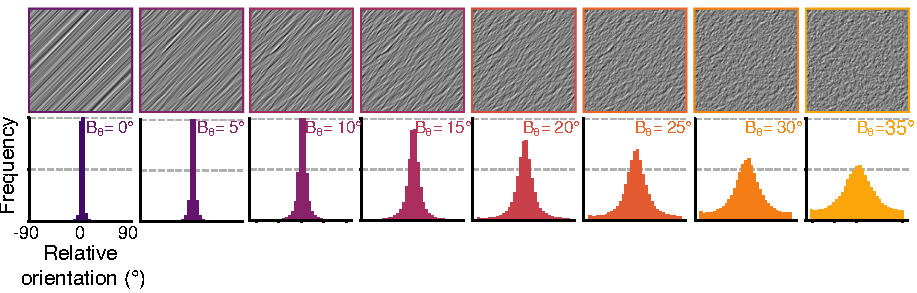
\includegraphics[width=.9\textwidth]{fig/chap2_fig_motionclouds.pdf}
\caption[An example of Motion Clouds.]{An example of Motion Clouds, with increasing orientation variance from left to right, and associated orientation distributions.}
\label{fig_chap2_stats_mc}
\end{figure}

Here, we will focus on the case of Motion Clouds, generative model-based stimuli~\cite{leon2012motion} which allow for fine parameterized control over a naturalistic stimuli~\cite{vacher2015biologically}, which is a desirable trait when probing sensory systems under realistic conditions~\cite{rust2005praise}. They are mathematically defined as band-pass filtered white noise stimuli, whose filters in Fourier space are defined as a parameterized distribution in a given perceptual axis (here, only orientation). 
Thus, the Motion Clouds presently used are fully characterized by their mean orientation and their orientation variance, such that a given stimulus $S$ can be defined as:

\begin{equation}
    \text{S} = \mathcal{F}^{-1} (O(\theta, B_{\theta}))
\end{equation}

where $\mathcal{F}$ is the Fourier transform and $O$ the orientation envelope, characterized by its mean orientation $\theta$ and its orientation bandwidth $B_\theta$. For $B_\theta < 45.0$°, a good approximation is $B_\theta = 1/\sqrt{\kappa}$, where $\kappa$ is the concentration parameter of a von Mises distribution (see below), and hence approximates the standard deviation~\cite{swindale1998orientation}. It thus serves as a measure of the orientation variability in the pattern, and as such, we will use the term "variance" to describe it throughout the thesis.
The orientation envelope is a von Mises distribution:
\begin{equation}\label{eq_orientation_mc}
O(\theta, B_{\theta}) = 
\exp 
\left\{
\frac{\cos (2 (\theta_f - \theta)) }
{4 \cdot B_{\theta}^2}
\right\}
\end{equation}
where $\theta_f$ is the angle of the frequency components of the envelope in the Fourier plane, which controls the spatial frequency parameters of the stimuli. For the range of values of $B_\theta$ considered in the present thesis, the orientation envelope approximates a Gaussian distribution and $B_\theta$ is thus a measure of the variance of the orientation content of the stimuli that follows a naturalistic distribution, as highlighted in chapters 3, 4 and 5. 

Such stimuli offer three advantages over both simple grating-like stimuli and complex natural images. First, they enable fine control of mean orientation, controlled by $\theta$, and its variance, controlled by $B_\theta$. This thus allows to reproduce natural images' oriented content, solely in terms of orientation distributions. Second, as they are stationary in the spatial domain, they only probe orientation space, excluding any second-order information exploitable by the visual cortex~\cite{johnson2004first}. Third, by conforming to natural images' $1/f^2$ power spectrum distribution~\cite{field1987relations}, they attain a desirable balance between controllability and naturalness~\cite{rust2005praise}. The combination of these traits allowed Motion Clouds to be successful in describing the perceptual integration of the human visual system~\cite{simoncini2012more}, the dynamical computations of retina~\cite{ravello2019speed}, and the dynamics of naturalistic perception in \gls{V1}~\cite{vacher2017synthese}. Controlling a naturalistic stimulus confers a significant benefit here, namely in allowing us to control the variance of these distributions, whose role in vision we will now explore.



\subsubsection{Variance in vision}
Herman von Helmholtz, in his treatise of physiological optics~\cite{helmholtz1925treatise}, gave a pinpoint accurate description of variance in sensory perception:
\begin{displayquote}
	“Given that the world we live in is loaded with statistical noise, [$\approx$ variance] expectations must be represented as part of the brain’s models.”
\end{displayquote}

Sources of variance are plentiful in vision (Figure \ref{fig_chap2_variance_psychophysics}). Well-known optical illusions demonstrate how an object can seem brighter than it actually is, when light intensity is juxtaposed against a dark background. Obstruction patterns lead us to inaccurately fill in parts of the visual field. Motion can blur our perception. Here, our primary interest lies in the orientation variance and its effect on vision, a sub-field that has been extensively explored psychophysically, yet remains relatively uncharted in terms of electrophysiological investigations.

\begin{figure}
\vspace{-0.25cm}
\centering
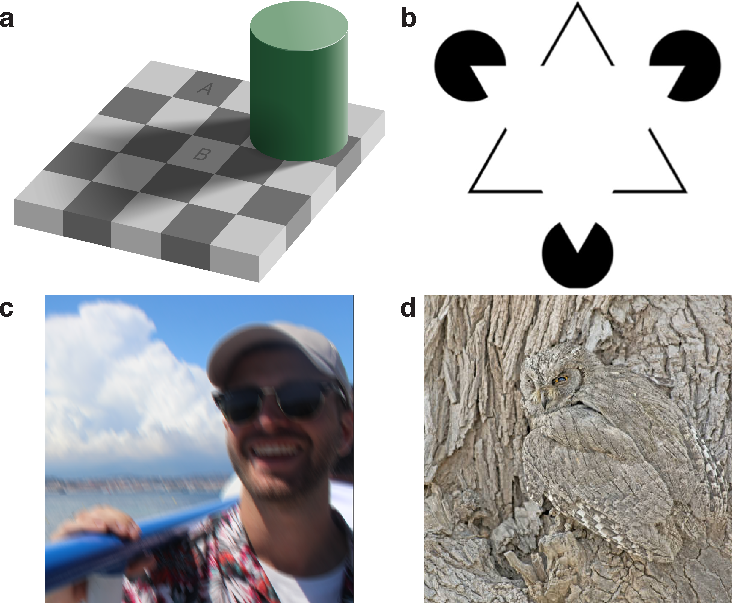
\includegraphics[width=.75\textwidth]{fig/chap2_fig_visionvariance.pdf}
\caption[Example of visual uncertainties.]{Example of visual uncertainties, on: (a) contrast, (b) obstruction, (c)  motion blur, (d) orientation (picture taken by \href{https://www.flickr.com/photos/noorhussain}{Noor Hussain}).}
\label{fig_chap2_variance_psychophysics}
\end{figure}

In psychophysics, variance is often interchangeably used with the term 'uncertainty'~\cite{szeliski1990bayesian}. In the context of orientation, the term 'bandwidth' is also often used, for historical reason~\cite{snowden1992orientation}, as studying a broadband signal in orientation domain is straightforward, and creating such a signal by blending point sources of orientation to generate a distribution is even simpler. In statistical term, one can also use inverse variance ($1/\sigma$) and its squared term, the precision ($1/\sigma^2$). Under Gaussian approximation, such as in chapter 3 and 4 (see also Equation~\ref{eq_orientation_mc}), bandwidth approximates variance, and both can be linked to inverse variance and precision through their straightforward mathematical relationship. Uncertainty, when used in this manuscript, will also refer to the notion of a "broader" distribution of features (often, of orientations). One could nonetheless be "certain" of a given large "variance", for example, by asking a human subject to judge the degree of variance of a given texture. That specific meaning will not be used in this manuscript (see for example~\cite{barthelme2009evaluation,geurts2021reported,sanchez2023action}), and we will refer to inverse variance and variance when describing the computations at play here.

The general study of orientation variance can be traced back to parametric texture generation, starting with Bela Julesz work on "textons"~\cite{julesz1981textons}. These simple oriented elements were shown to human subjects, and shown to take an increasingly great amount of time to process as their complexity (i.e. variance in orientation space) increases~\cite{julesz1983human}.
Under different texture synthesis algorithms and experimental paradigms, this observation has been replicated a number of time, showing that the impact of increasing variance on orientation detection is rather intuitive: as variance rises, performance deteriorates~\cite{phillips1984orientation,heeley1989width,heeley1998influence}. This is a non-linear effect~\cite{heeley1998influence} that works similarly to contrast response curve. Computationally, it is well accounted for by models of recurrent cortical activity~\cite{keeble1995detection,beaudot2006orientation}, and more specifically the result from the competition among multiple orientation detectors~\cite{ringach2002orientation}.

This is however not a mere passive influence, but an active mechanism, accounted for by human observers~\cite{barthelme2009evaluation}. This behavior aligns with Bayesian models of perception, which, as we will discuss in the upcoming algorithmic section of the introduction, is of central importance for our work. Briefly, a Bayesian account of perception implies an active encoding of variance in the brain, granting access to this information for decision-making~\cite{geurts2022subjective}. For instance, let us imagine an observer walking through a forest and hearing leaves rustling. If one's vision is clear, and one spots a squirrel, they'd likely carry on without concern. However, if their vision is obstructed by dense bushes (creating an increased orientation variance), they'd likely rely more heavily on their internal priors, which in most instances, would dictate a cautious retreat. Vision does not work as passive acceptance of uncertain input, but rather, requires our brain to cross-reference what it sees with a prior model of the world.

Despite the convergence psychophysical accounts and theoretical requirements, there is a significant gap in the literature on the implementation of variance computations in the brain~\cite{koblinger2021representations}. This discrepancy could be attributed to the complexities involved in applying parametric texture synthesis to probe the visual system, making electrophysiological investigations challenging. As this section of the introduction primarily focuses on the computational level, we direct the reader to the concluding part of the introduction for a detailed explanation of the implementational mechanisms of variance within the brain, and now turn our attention to describing the basic requirements for variance-based in computations.



\newpage 



\subsection{The algorithmic level: A probabilistic model of perception}
Marr's second level, the algorithmic level, is concerned with the operations that the system performs, and how these are organized to realize the computations described at the previous level. This section aims to describe probabilistic operations that can account for visual tasks, adopting an iterative approach to the problem of perception. We will follow the common formalism and mathematical development for this class of problem~\cite{bogacz2017tutorial}, framed with additional justifications of equations and examples fitted to the problem under study.

\subsubsection{A simple example of Bayesian Inference}
We start by considering a simplistic toy example in which an organism is tasked with inferring a single variable, the size of a food item denoted by $v$, based on a single observation, the light intensity denoted by $u$. The organism's sensory input is constrained, as ours, to be noisy~\cite{barlow1956retinal}, such that the true item size $v$ is normally distributed based on observations $u$. Given that light reflections are related to the surface of the object, let's consider a distribution with a mean true item size $g(v)$, where $g(v) = v^2$, and a variance based on noise on observations $\Sigma_u$. This is expressed as:

\begin{equation}\label{eq_proba_intro}
    p(u|v) = f(u;g(v), \Sigma_u) = \frac{1}{\sqrt{2\pi\Sigma_u}} exp{\frac{(u-g(v))^2}{2\Sigma_u}} 
\end{equation}

Given this probabilistic description of the input and the arguments previously stated in favor of vision as a probabilistic process, we shall also describe such organism as performing probabilistic inference. We thus consider that this organism has had the chance of encountering many food items in his life, and that it can implement prior expectation $p(v)$ about the size of the food item. This is also normally distributed, with mean $v_p$ and variance $\Sigma_p$:

\begin{equation}
p(v) = f (v; v_p, \varSigma_p) = \frac{1}{\sqrt{2\pi\Sigma_v}} \exp{\frac{(v-v_p)^2}{2\Sigma_p}}
\end{equation}

Given this framework, we can apply Bayes' theorem to compute an exact solution to the inference problem based on a single observation of light intensity, which is given by:

\begin{equation}
\label{eq_denominator}
p(v|u) = \frac{p(v)p(u|v)}{p(u)} = \frac{\frac{1}{\sqrt{2\pi\Sigma_p}} \exp{\frac{(v-v_p)^2}{2\Sigma_p}} \frac{1}{\sqrt{2\pi\Sigma_u}} \exp{\frac{(u-g(v))^2}{2\Sigma_u}}}{\int p(v) p(u|v)dv}
\end{equation}

The numerator term is simply the product of the prior and the likelihood described above. The normalization term, however, is more complex. It is the integral of all $p(v)p(u|v)$, which ensures that the posterior probabilities of $p(v|u)$ sum to $1$, but is too computationally intensive for a realistic system, as it would require sampling all possible configurations of the problem. This consideration is left to the implementational level of the introduction, and does not deter us presently from computing an exact solution using Bayes' theorem. This yields the graphical representation of integrating likelihood $p(u|v)$ and prior $p(v)$ into a posterior distribution $p(v|u)$. 

\begin{figure}[h!tbp]
\vspace{0.5cm}
\centering
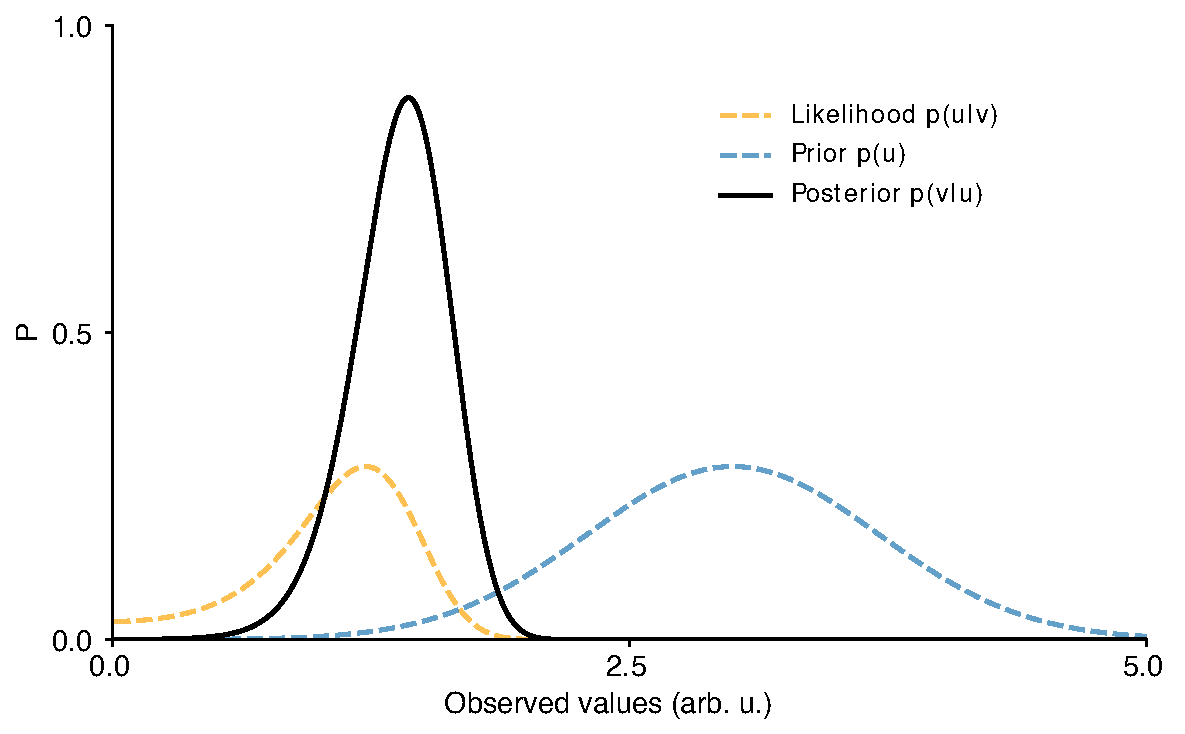
\includegraphics[width=.9\textwidth]{fig/chap2_fig_equi_proba.pdf}
\caption[A simple example of Bayesian integration.]{A simple example of Bayesian integration. Integrating observed (likelihood) and former (prior) distributions, with $\Sigma_u = \Sigma_p = 0.5$. The most likely value of $v$ lies between the two distributions.}
\label{fig_chap2_equi_proba}
\end{figure}

Through the representation of Figure \ref{fig_chap2_equi_proba}, one can notice how non-intuitive and non-linear Bayesian inference can be, even in such a simple example framed here. For the organism that must estimate $p(v|u)$, once the (input) likelihood $p(u|v)$ involved becomes a non-standard distribution, it becomes necessary to represent infinitely many $p(v|u)$ values for many possibles $v$, rather than first order statistics like mean and variance. As we've said, however, this would require infinitely too many computations for a biological system. Instead of computing the whole distribution, this organism could try to maximize the value of $p(v|u)$, in order to infer the most likely value of $v$. This procedure is called \textit{maximum likelihood estimation} and involves sampling a posterior distribution $p(\Phi | u)$ of the most likely size $\Phi$:

\begin{equation}
\label{eq_MLE}
p(\phi|u) = \frac{p(\phi)p(u|\phi)}{p(u)}
\end{equation}

As the denominator does not depend on $\Phi$, we focus on the numerator. We will denote its logarithm $F$, as it relates to the Free Energy described later:

\begin{equation}
     F = \ln  \left( p(\Phi) p(u|\Phi) \right) = \ln p(\Phi) + \ln p(u|\Phi)
\end{equation}

The natural logarithm having removed the exponential terms involved in Equation~\ref{eq_denominator}, we get: 
\begin{equation}
\label{eq_F}
  \begin{aligned}
    F & = \ln p(\Phi) + \ln p(u|\Phi) \\ 
      & =\ln \left( \frac{1}{\sqrt{2\pi\Sigma_p}} \exp{-\frac{(\Phi-v_p)^2}{2\Sigma_p}}\right) + \ln \left( \frac{1}{\sqrt{2\pi\Sigma_u}} \exp{-\frac{(u-g(\Phi))^2}{2\Sigma_u}} \right) \\
      & = \ln \left( \frac{1}{\sqrt{2\pi\Sigma_p}} \right) + \ln \left(\exp{-\frac{(\Phi-v_p)^2}{2\Sigma_p}} \right) + 
            \ln \left( \frac{1}{\sqrt{2\pi\Sigma_u}} \right) + \ln \left(\exp{-\frac{(u-g(\Phi))^2}{2\Sigma_u}} \right) \\
      & = \ln \left( \frac{1}{\sqrt{2\pi}} \right) - \frac{1}{2} \ln \Sigma_p- \frac{(\Phi-v_p)^2}{2\Sigma_p} + 
            \ln \left( \frac{1}{\sqrt{2\pi}} \right) - \frac{1}{2} \ln \Sigma_u -  \frac{(u-g(\Phi))^2}{2\Sigma_u} \\ 
      & =  \frac{1}{2} \left( - \ln \Sigma_p - \frac{(\Phi - v_p)^2}{\Sigma_p}  - \ln \Sigma_u - \frac{(u - g(\Phi))^2}{\Sigma_u}\right) + C
  \end{aligned}
\end{equation}

Now, it is simpler to find the derivative of $F$ to look for a maximum value of our food estimate posterior distribution, we can compute the derivative of $F$ over $\Phi$ (as done in Appendix \ref{appendix_maths}), we get:

\begin{equation}
\label{eq_dF_dPhi}
    \frac{\delta F}{\delta \Phi} = \frac{(u-g(\Phi))}{\Sigma_u} g'(\Phi)  + \frac{(v_p-\Phi)}{\Sigma_p}  
\end{equation}
which endows our example organism with the ability to find the most likely value of the food item size $v$ by varying $\Phi$ with respect to the sign of the derivative. The first term of the equation drives the posterior distribution towards the likelihood, and the second one towards the prior, both of which are weighted by the inverse of their respective variance, $\Sigma$.
This equation is central to the remainder of this algorithmic part of the introduction, and really to this entire thesis, as it provides a mathematical role for variance in (visual) perception. It can be easily tied, in this form, to the Free Energy principle, introduced in the next section.



\subsubsection{Free Energy principle for variational inference}
The free energy principle allows both to understand how complex systems can model the most likely values of variables, as above, but also their distribution, as is the goal of this thesis. Briefly, this theory traces its roots to the work of Hermann von Helmhotz' unconscious inference~\cite{helmholtz1925treatise}, who was arguably the first physiologist to propose the notion that the mind construct a perception of the world through probabilistic inference. The idea of free energy in the brain gained popularity through the seminal works of Karl Friston~\cite{friston2006free, karl2012free, aguilera2022particular}, who also proposed its realization in the form of a neuroscience theory called predictive coding~\cite{friston2005theory, friston2009predictive}. In this section, we shall dive into the details of variational free energy, a specific formulation of free energy that will allow us to formulate general equations on which the rest of the thesis will rely.

In the text preceding Equation \ref{eq_MLE}, we mentioned that posterior distributions $p(v|u)$ can have complex shapes that mandate prohibitively dense sampling for many values of $u$. As an approximation to avoid this issue, we proposed the method of sampling solely the maximum of these distributions. However, it is beneficial to know the shape of the full distribution, namely for knowing the variance - and thus the reliability - of estimates~\cite{mansournia2016inverse}, as we wish to see in neurobiological systems in this thesis. An improved solution of maximum likelihood estimate is an alternative approach that involves the utilization of a "surrogate" distribution, in a process called variational inference~\cite{murphy2012machine}. This distribution, which we will refer to as $q(v)$, possesses a standard form that can be succinctly described by its mean and variance, unlike the distribution it surrogates in the first place.
To approximate our complex posterior $p(v|u)$ with $q(v)$, we need a metric of (dis)similarity between the two distributions. For probability distribution and without particular assumptions, the choice is naturally the \gls{KL} divergence, defined as: 

\begin{equation}
KL(q(v), p(v|u)) = \int{q(v) \ln \frac{q(v)}{p(v|u)} dv}
\end{equation}

This divergence, or distance, is not symmetric, meaning that the divergence from $p(v|u)$ to $q(v)$ is not the same as the divergence from $q(v)$ to $p(v|u)$. This characteristic makes it particularly suitable for our purpose, as it allows us to measure how much information is lost when we use the surrogate function $q(v)$ to approximate the original distribution $p(v|u)$. By minimizing the \gls{KL} divergence, we can ensure that our surrogate function is as close as possible to the original distribution, thereby providing a more accurate and efficient representation of the complex posterior distribution.

As is, this approach doesn't make things any easier, as we are still required to calculate the same normalization term as in Equation \ref{eq_denominator}, a barrier that led us to maximum likelihood estimate in the first place. This is where the concept of Free Energy proves to be immensely beneficial.
By definition, we already know that:

\begin{equation}
    p(v|u) = \frac{p(u, v)}{p(u)}
\end{equation}

which we can use into the equation of the \gls{KL} divergence as:

\begin{equation}
    \begin{aligned}
        KL(q(v), p(v|u)) & = \int{q(v) \ln \frac{q(v)}{p(v|u)} dv} \\ 
                        &= \int{q(v) \ln \frac{q(v)p(u)}{p(u,v)} dv} \\
                        &= \int{q(v) \ln \frac{q(v)}{p(u,v)} dv} + \int{q(v) \ln p(u) dv} \\
    \end{aligned}
\end{equation}

given that $q(v)$ is a probability distribution and sums up to $1$, we thus obtain:

\begin{equation}
    KL(q(v), p(v|u)) = \int{q(v) \ln \frac{q(v)}{p(u,v)} dv} + \ln p(u) \
\end{equation}

by defining the variational free energy as the negative of the term that is concerned with our surrogate distribution, we get:

\begin{equation}
\label{eq_free_energy_KL}
    \begin{aligned}
        F &= \int q(v) \ln \frac{p(u,v)}{q(v)} dv, \\
        KL (q(v), p(v|u)) &= -F + \ln p(u)
    \end{aligned}
\end{equation}

since only $F$ pertains to our surrogate distribution $q(v)$, the parameters of this function that minimize the divergence between $q(v)$ and the actual posterior $p(v|u)$ are the same as those that maximize $F$. Note that this $F$ denotes that variational free energy, that is, the free energy involved in this approximation process, and not the general free energy of the system. To obtain the best surrogate distribution to approximate the posterior, we can now simply maximize $-F$, which does not involve the complex computation of the normalization term. In the next section, this will also serve to introduce learning of parameters of models. As we shall soon see, such learning involves, intuitively, being wrong as rarely as possible in our inference process. In other term, we wish to minimize the surprise, as defined by Shannon~\cite{shannon1948mathematical}, associated with our predictions. Given Equation \ref{eq_free_energy_KL}:

\begin{equation}
\label{eq_lnpu}
    - \ln p(u) = F+ KL (q(v), p(v|u)) 
\end{equation}

As the \gls{KL} divergence is positive, $F$ can only be a lower bound of $\ln p(u)$. Maximizing the variational free energy $F$ thus minimizes surprise $\ln p(u)$, meaning that we improve the approximation of $q(v)$ and thus optimize our internal model using this simple framework.



\subsubsection{Prediction errors under the free energy principle}
As we are progressively moving from the algorithmic to the implementation level, our formulation of Bayesian inference under the Free Energy principle could use a reframing more related to neurobiology. In that sense, this section of introduction will tell us now how to formulate Bayesian inference in simpler terms, and second how to derive learning rules. 

Going back to Equation \ref{eq_dF_dPhi}, we showed that deriving the parameter $\Phi$ could be written as:

\begin{equation}
    \frac{\delta F}{\delta \Phi} = \frac{(u-g(\Phi))}{\Sigma_u} g'(\Phi)  + \frac{(v_p-\Phi)}{\Sigma_p}  
\end{equation}

we can now perform some helpful variable renaming, with the left-hand side of the equation becoming:

\begin{equation}
    \epsilon_p = \frac{(v_p-\Phi)}{\Sigma_p} 
\end{equation}

and the rest being:

\begin{equation}
    \epsilon_u = \frac{(u - g(\Phi))}{\Sigma_u}
\end{equation}

such that the derivative becomes:
\begin{equation}
\frac{\delta F}{\delta \Phi} = \epsilon_u  g'(\Phi)   + \epsilon_p 
\end{equation}

and the update rule of $\Phi$ to follow the gradient of $F$ is then:

\begin{equation}
    \dot{\Phi} = \epsilon_u  g'(\Phi) - \epsilon_p
\end{equation}

Both $\epsilon_p$ and $\epsilon_u$ measure the difference between a real and inferred value, and are thus both called prediction errors~\cite{friston2005theory} (hence the term predictive coding). The term $\epsilon_p$ is often referred to, in the literature~\cite{millidge2021predictive}, as the prediction error on the causes, and measures the difference between the inferred observation and the model's prior expectations. The term $\epsilon_u$, on the other hand, is called the prediction error on the states, and measures the difference between the observed value and the inferred value. In predictive coding, the goal of a model is to minimize both sources of prediction errors, and as such it needs a learning rule based on prediction errors. When looking for the point at which the system's prediction error become null, we get the stable point of $\epsilon_p$:

\begin{equation}
    \begin{aligned}
        \epsilon_p &= \frac{\Phi - v_p}{\Sigma_p} \\
        \Sigma_p\epsilon_p &= \Phi - v_p \\
        \Phi - v_p - \Sigma_p\epsilon_p &= 0 
    \end{aligned}
\end{equation}

and the one of $\epsilon_u$:

\begin{equation}
    \begin{aligned}
        \epsilon_u &= \frac{u - g(\Phi)}{\Sigma_u} \\
        \Sigma_u\epsilon_u &= u - g(\Phi)\\
         u - g(\phi) - \varSigma_u \varepsilon_u &= 0
    \end{aligned}
\end{equation}

And thus the dynamics of a system that seeks to minimize its prediction errors can be described as: 

\begin{equation}
\begin{aligned}
\dot{\varepsilon_p} &= \phi - v_p - \varSigma_p \varepsilon_p  \\
\dot{\varepsilon_u} &= u - g(\phi) - \varSigma_u \varepsilon_u  \\
\end{aligned}
\end{equation}

This is however not an ideal description, because it assumes the rest of the parameters of the system $v_p, \Sigma_p, \Sigma_u$ are constrained. It becomes even more inconvenient in a thesis about the implementation of dynamical computations on $\Sigma$ parameters. This is where the free energy principle becomes extremely useful, as it ascribes a goal to the model: modifying parameters such that visual input $u$ becomes the least surprising. As described in Equation \ref{eq_denominator}, this is a term that involves the computation of a complex integral, but its natural logarithm can be more easily computed as in Equation \ref{eq_lnpu}, and even more so with $F$ defined in Equation \ref{eq_F}:

\begin{equation}
\begin{aligned}
    \ln p(u) & = F+ KL (q(v), p(v|u)) \\
            & = \frac{1}{2} \left[ - \ln \Sigma_p - \frac{(\Phi - v_p)^2}{\Sigma_p}  - \ln \Sigma_u - \frac{(u - g(\Phi))^2}{\Sigma_u}\right] + C + KL (q(v), p(v|u))
\end{aligned}
\end{equation}

as the \gls{KL} divergence is a strictly positive term that forms a lower bound on surprise, we will include it in the constant $C$ term for simplicity's sake. Following the (lenghty) derivations in Appendix \ref{appendix_maths} of $F$ over $v_p, \Sigma_p, \Sigma_u$, we get the following dynamics of our inference model:

\begin{equation}
\label{eq_df_derror}
    \begin{aligned}
    \frac{\delta F}{\delta v_p} &= \frac{\Phi - v_p}{{\Sigma_p}} \\
    \frac{\delta F}{\delta \Sigma_p} &= \frac{1}{2} \left[ \frac{(\Phi - v_p)^2}{{\Sigma_p^2}} - \frac{1}{{\Sigma_p}} \right] \\
    \frac{\delta F}{\delta \Sigma_u} &=  \frac{1}{2} \left[ \frac{(u - g(\Phi))^2}{{\Sigma_u^2}} - \frac{1}{{\Sigma_u}} \right]
    \end{aligned}
\end{equation}

by re-expressing these equations using the definition of prediction error as before, we get:

\begin{equation}
\label{eq_df_derror_final}
    \begin{aligned}
    \frac{\delta F}{\delta v_p} &= \frac{\Phi - v_p}{{\Sigma_p}} = \epsilon_p \\
    \frac{\delta F}{\delta \Sigma_p} &= \frac{1}{2} \left[ \frac{(\Phi - v_p)^2}{{\Sigma_p^2}} - \frac{1}{{\Sigma_p}} \right]  = \frac{1}{2} \left(\epsilon_p^2 - {\Sigma_p^{-1}} \right) \\
    \frac{\delta F}{\delta \Sigma_u} &=  \frac{1}{2} \left[ \frac{(u - g(\Phi))^2}{{\Sigma_u^2}} - \frac{1}{{\Sigma_u}} \right] = \frac{1}{2} \left(\epsilon_u^2 - {\Sigma_u^{-1}} \right)
    \end{aligned}
\end{equation}

where ${\Sigma^{-1}}$ denotes the inverse variance of a prediction error. This way of expressing predictive coding models shall be used in the reminder of the thesis, hence the need for a logical progression of $26$ equations to lay solid foundations to the rest of the manuscript. As we will see in the implementation section of this introduction, this expression possesses the desirable attribute of requiring only local variables, making it compatible with Hebbian learning rules~\cite{hebb1949organization}. Now that we have established a set of robust equations, we can commence our exploration into the crux of the issue: variance terms.

\subsubsection{On the specific case of variance}
A central aspect of predictive coding, which is often overlooked in the literature~\cite{rao1999predictive, Zongker2006, spratling2017hierarchical, wen2018deep, millidge2020relaxing} or reduced to identity matrices, is the variance term in Equation \ref{eq_df_derror_final}. As we have seen in the previous pages, this term naturally comes into play in Bayesian inference, and possesses a crucial role in driving the dynamics of a model, driving the posterior distribution of a system closer or further from the likelihood.

\begin{figure}[h!tbp]
\vspace{0.5cm}
\centering
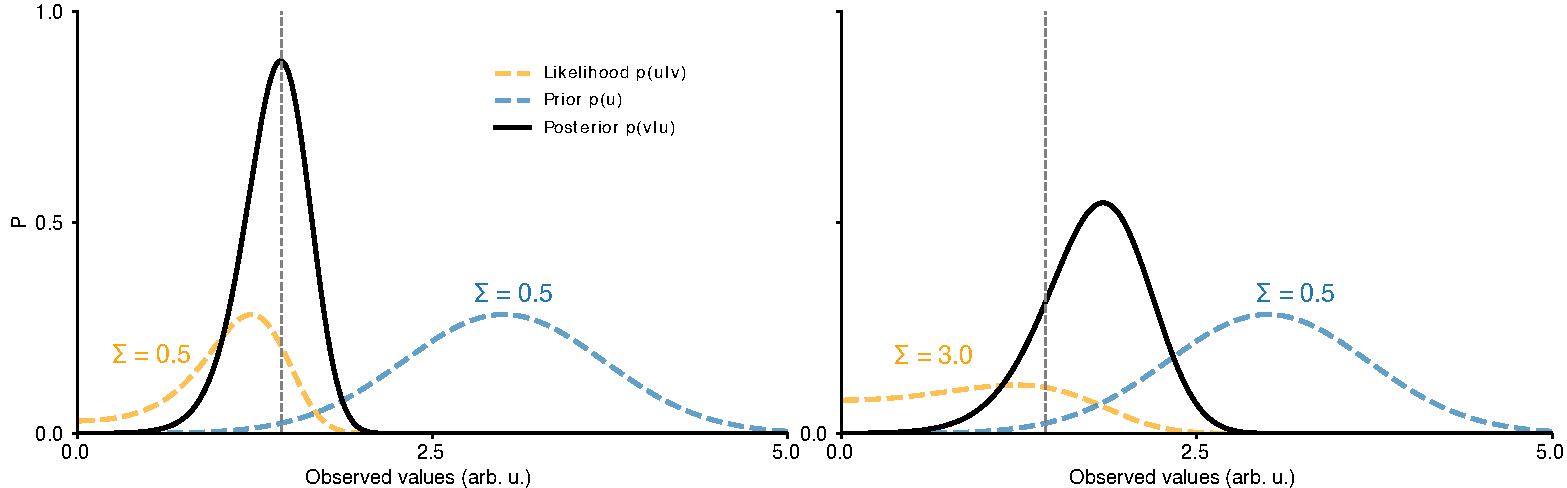
\includegraphics[width=1.\textwidth]{fig/chap2_fig_equi_proba_var.pdf}
\caption[The role of variance in Bayesian integration.]{The role of variance in Bayesian integration. (left) As in Figure \ref{fig_chap2_equi_proba}, Bayesian integration with $\Sigma_u = \Sigma_p = 0.5$. The most likely value of $v$ is indicated by a gray dashed line. (right) Same but with $\Sigma_u = 6\Sigma_p$, driving the posterior away from the sensory likelihood.}
\label{fig_chap2_equi_proba_var}
\end{figure}

This relates to a number of fascinating emergent properties in neural system which will be discussed in later parts of the introduction, namely of neuromodulation~\cite{friston2005theory}, attention~\cite{kanai2015cerebral} and even psychiatric disorders~\cite{adams2013computational, perrinet2014active}. This also speaks of a hierarchy of prediction and prediction errors, whose multiple integration levels are driven by the relative variance of external inputs and internal predictions. Whilst this is discussed more in details in the implementation part of the introduction, we can already state that low-level prediction errors, like the one encoded in \gls{V1}, are tightly bound to the variance of the sensory input, and computationally, learning such variance allows to learn about the extrinsic variability of the external world (see chapter 3). This also allows the visual system to factor in the intrinsic variability of its sensors~\cite{faisal2005ion, faisal2008noise}. 

We shall see in the coming section that the abundance of generic ideas about variance is counterbalanced by the lack of specific neurobiological and neurocomputational literature at the implementational level. As this portion of the introduction is exclusively focused on algorithmic-level concepts, we will not delve deeper into variance at this point. Instead, we will now be focused on computations that can be done on the variance of sensory input, i.e. the likelihood $p(u|v)$.



\newpage 



\section{The two-fold approach to the problem under study}
Having clarified the computational 'why' and algorithmic 'what' of our undertaking, we now turn to the 'how' of its implementation - Marr's final level of analysis, the implementational level, a final stage where our theoretical statements comes to fruition. As previously done, this section aims to provide an overview of the relevant parts of the literature whilst refraining from being a bullet-point detailed list. This is especially the case in the neurobiological section of this introduction, which is concerned with the actual realization of our theories, rather than their experimental aspects, which will be reserved for the introduction of their respective chapters.



\subsection{The in-silico implementational level: Neurocomputations}
The first part of this introduction to the implementational level involves transitioning from the theoretical underpinnings of predictive coding under the free energy principle, towards a practical model that can effectively be employed in vision.



\subsubsection{Predictive coding for vision}
As stated in Equation \ref{eq_df_derror_final}, every single variable required by our formulation of predictive coding can be expressed in terms of a graph with local variables. Such network can be represented as in Figure \ref{fig_chap2_pc_graphs}.

\begin{figure}[h!tbp]
\vspace{0.5cm}
\centering
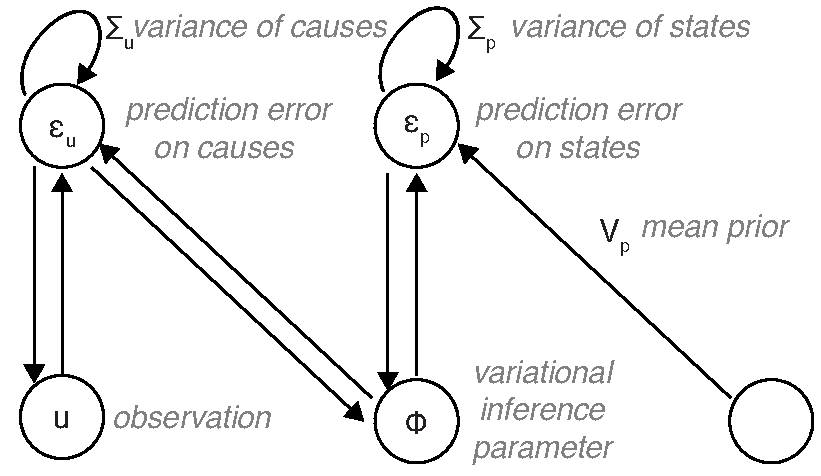
\includegraphics[width=.85\textwidth]{fig/chap2_fig_pc_graph.pdf}
\caption[A simple predictive coding graph.]{A simple predictive coding graph, with helpful reminder of the variables nomenclature in gray.}
\label{fig_chap2_pc_graphs}
\end{figure}

This network constitutes what is known as an acyclic computational graph, a generalized method of articulating problems to topology that will prove useful in chapter~5. Empirical studies have also shown that predictive coding can perform on par (or even better) than the main method of training deep neural networks along such a graph~\cite{millidge2022predictive}, a method known as backpropagation~\cite{lecun1989backpropagation}. This important property helps us scale such a graph beyond the unidimensional form, as we have been doing so far, to a form where "nodes" of the graphs (neurons) would for example represent multiple different orientation in the visual field, as in Figure \ref{fig_chap2_pc_matrix_graphs}.

\begin{figure}[h!tbp]
\vspace{0.5cm}
\centering
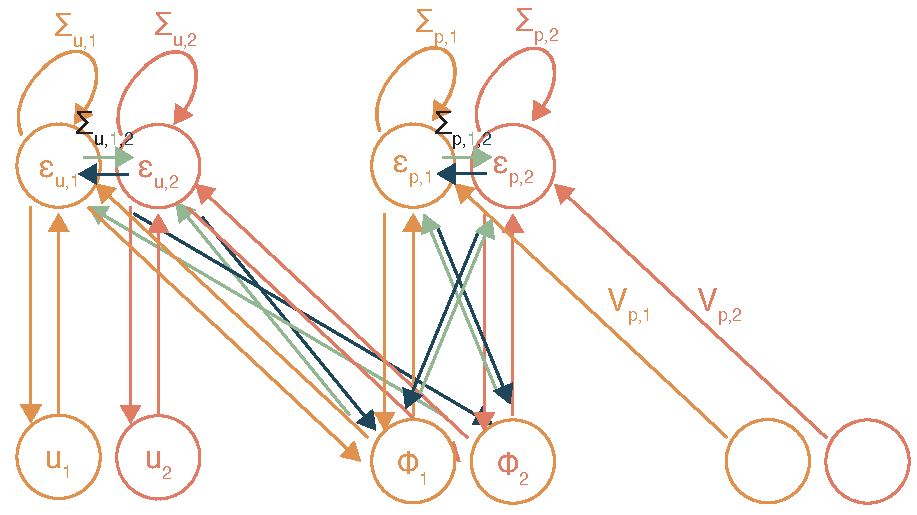
\includegraphics[width=.85\textwidth]{fig/chap2_fig_pc_graph_matrix.pdf}
\caption[A matrix form predictive coding graph.]{A matrix form (with two elements) of the previous predictive coding graph, with additional inter-matrix elements connections colored in green and dark blue.}
\label{fig_chap2_pc_matrix_graphs}
\end{figure}

Following the derivations of Appendix~\ref{appendix_maths}, such network then becomes, in matrix notation, where $\mathit{x}$ is a scalar, $\bar{x}$ a vector and $\mathbf{x}$ a matrix:
\begin{equation}
    \begin{aligned}
       \dot{\bar{\varepsilon}}_p &= \bar{\phi} - \bar{v}_p - \mathbf{\Sigma_p}\bar{\varepsilon}_p \\
       \dot{\bar{\varepsilon}}_u &= \bar{u} - g(\bar{\phi}) - \mathbf{\Sigma_u}\bar{\varepsilon}_u
    \end{aligned}
\end{equation}

with the dynamics of the matrices being:
\begin{equation}
\label{eq_pc_matrix}
    \begin{aligned}
        \frac{\delta F}{\delta \bar{v_p}} &= \bar{\epsilon}_p \\
        \frac{\delta F}{\delta \boldsymbol{\Sigma_p}} &= \frac{1}{2}(\bar{\epsilon}_p\bar{\epsilon}_p^T - \boldsymbol{\Sigma_p^{-1}}) \\
        \frac{\delta F}{\delta \boldsymbol{\Sigma_u}} &= \frac{1}{2}(\bar{\epsilon}_u\bar{\epsilon}_u^T - \boldsymbol{\Sigma_u^{-1}})
    \end{aligned}
\end{equation}

This approach is extremely useful to us, as it allows us to incorporate multiple sensory inputs to the network, like multiple oriented edges to \gls{V1}, which is a critical aspect of the implementational challenge in this thesis. Sadly, it also introduces a major complication, because the inverse variances represented by $\boldsymbol{\Sigma^{-1}}$ now require matrix inversion. This necessitates a network-wide computation, implying that all nodes must access the entirety of the data instantaneously, which is not biologically plausible. Further, such matrix inversion is computationally demanding~\cite{csanky1975fast}, which is one reason why inverse variance weighting is mostly absent from existing predictive coding implementations.
This now presents us with the first implementational issue related to the computations we have detailed so far: trying to incorporate the algorithms we have designed into a formulation that is biologically plausible. While numerous solutions exist~\cite{friston2005theory, bogacz2017tutorial, kanai2015cerebral}, we shall continue one that is naturally suited to matrix forms~\cite{bogacz2017tutorial} and involves the addition of an extra inhibitory neuron, as in Figure \ref{fig_chap2_pc_matrix_graphs_inhibitory}.

\begin{figure}[h!tbp]
\vspace{0.5cm}
\centering
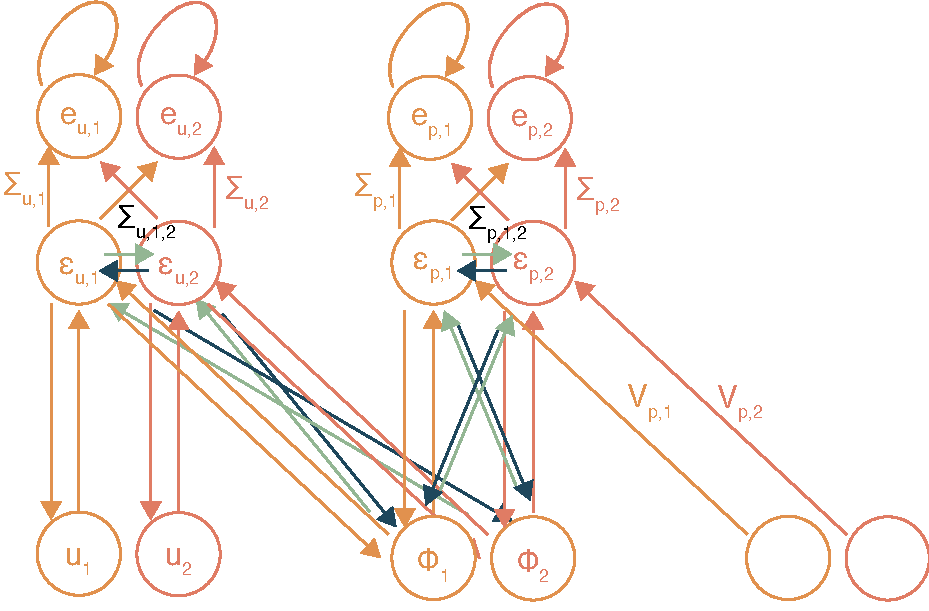
\includegraphics[width=.8\textwidth]{fig/chap2_fig_pc_graph_matrix_hebbian.pdf}
\caption[A matrix form predictive coding graph with Hebbian variables.]{A matrix form predictive coding graph with Hebbian variables.}
\label{fig_chap2_pc_matrix_graphs_inhibitory}
\end{figure}

Based on the notions developed in the final section of Appendix \ref{appendix_maths}, the equation of the prediction errors of the network thus becomes:
\begin{equation}
    \begin{aligned}
\dot{\bar{\varepsilon}}_p &= \bar{\phi}_p - g(\bar{\phi}_{i+1}) - \bar{e}_p  \\
\dot{\bar{e}}_p &= \mathbf{\Sigma_p} \bar{\varepsilon}_p - \bar{e}_p 
    \end{aligned}
\end{equation}
where $e_i$ represents the additional inhibitory neuron. This implementation answers our needs for being able to handle the uncertain nature of vision through learned $\Sigma$ matrices, as detailed in the computational part of the introduction, while also being able to transcribe all the equations of the computational part of the introduction into a tangible and useful form.

But where does the "predictive" aspect of this predictive coding stem from ? This type of modelling can be traced back to \gls{V1} models developed by Rao and Ballard~\cite{rao1999predictive}, who transformed what was originally a signal processing algorithm developed for unidimensional signals~\cite{makhoul1975linear} into arguably one of the most robust theories in neuroscience~\cite{friston2009predictive}. By deriving the principle of efficient coding~\cite{barlow2001redundancy}, they reasoned that neural networks can all be described as predictive networks, like the one formulated above, and can serve as excellent models for \gls{V1}. This proved to be groundbreaking, even predicting the existence of non-classical phenomena~\cite{rao1999predictive} that previously required dedicated models~\cite{skottun1998model}. The remarkable simplicity and beauty of this approach, carried by the free energy principle, is well captured by a quote from Karl Friston~\cite{friston2018does}:
\begin{displayquote}
''Every decade or so, one reads a paper that makes you think “well, that’s quite remarkable”. [Rao and Ballard] showed that a simple architecture was not only consistent with neuroanatomy and physiology but could also account for a range of subtle response properties [...] \\
This was a significant achievement in its own right; however, the really remarkable thing —at least for me— was the following: in simulating their little piece of synthetic cortex, neuronal dynamics and connectivity optimized the same energy or cost function.''
\end{displayquote}

This breakthrough sets the stage for the tremendous success of predictive coding in artificial neural networks. Such predictive network perform on par with deep neural networks, can classify images datasets, predict complex natural images sequences, among many other remarkable feats. Unfortunately, the inclusion of variance is often overlooked in the implementation of such networks. This is not only due to the added complexity it brings to an already intricate network, but also because most of these networks employ point-based estimates rather than comprehensive Bayesian-like distribution learning. Such gap is exactly the aim of this thesis.

One exceptional aspect of predictive coding, though not extensively addressed in this thesis, is the fundamental idea that the brain must predict its inputs and possess a generative model of the world to account for its interpretations. What amplifies the significance of this is the fact that these generative models are self-invertible~\cite{millidge2021predictive}: practically speaking, one can train them, for instance, to classify objects, then simply reverse the flow of information and have them transformed into generative models of images~\cite{millidge2020relaxing}. An example of this reversal can be found at our \href{https://github.com/neuromorphs/BrainDishSiMulator/blob/main/notebooks/Dishbrain_predictive_coding.ipynb}{GitHub repository}, detailing the work we conducted at Telluride workshop to use predictive (generative) coding models in order to issue commands to in-vitro neurons.

In light of this series of generative/discriminative model, predictive coding also suggests a hierarchical series of explanations, which aligns remarkably well with the hierarchical nature of visual processes~\cite{boutin2021sparse, boutin2022pooling}. At the scale of our focus on \gls{V1}, predictive coding is particularly impactful as there have been numerous attempts to align the computations performed within the cortical "microcolumn" circuits, or microcircuits, with those carried out by predictive coding~\cite{bastos2012canonical}. This serves as the starting point for our bridge towards the biological aspect of our networks~\cite{shipp2016neural}, by employing such theories as a lens to delve into the cortex.

\newpage

\subsubsection{Microcircuits as a bridge from the theory to the cortex}
Having now expressed the problem of probabilistic vision in a form that can be mapped onto a graph, the next step is to transpose that graph into a neural network. In the introductory section related to the neurobiology of vision, we discussed some (controversial~\cite{horton2005cortical}) attempts to identify a recurring circuit in the cortex~\cite{douglas1989canonical, douglas2004neuronal}. As a reminder, such "canonical microcircuit" tracks the flow of information through multiple neurons, and was first established through intracellular recording in the cat's \gls{V1}~\cite{douglas1989canonical} to measure pre- and post-synaptic connectivity and functional strength. According to these studies and others~\cite{thomson2002synaptic}, a feedforward flow of excitatory activity in the cortical microcolumn arises from thalamic inputs to layer IV, then to layer II/III, and finally back to layer V/VI. There is proof that other excitatory pathways that would close the loop only form a minority of connections, namely the layer II/III to layer IV or layer V to layer II/III~\cite{thomson2002synaptic}. Inhibitory pathways in cortical microcolumn are historically harder to make out, namely because such neurons have much more functional subtypes~\cite{gouwens2019classification}, but recent evidences are showing that they can participate in the regulation of the circuit in a layer-specific fashion~\cite{bugeon2022transcriptomic}. Extrinsically, this circuit needs also to be integrated into an input/output scheme compatible with the idea of hierarchical predictive coding~\cite{boutin2022pooling}. Inhibitory connections play here an important role, because they allow multiple such microcircuit to compete against one another at the level of a cortical area~\cite{coultrip1992cortical, chavane2022revisiting} (see also chapter 4). At the macroscale level, backed by anatomical evidence~\cite{markov2014anatomy}, the final concept of a canonical microcircuit is that layer II/III sends synapses to higher order cortical areas~\cite{felleman1991distributed}, as opposed to layer V/VI that sends synapses to lower levels~\cite{markov2011weight}. Based on these considerations, Bastos et al.~\cite{bastos2012canonical} proposed a mapping of our computational graph onto a neural network:

\begin{figure}[h!tbp]
\vspace{0.1cm}
\centering
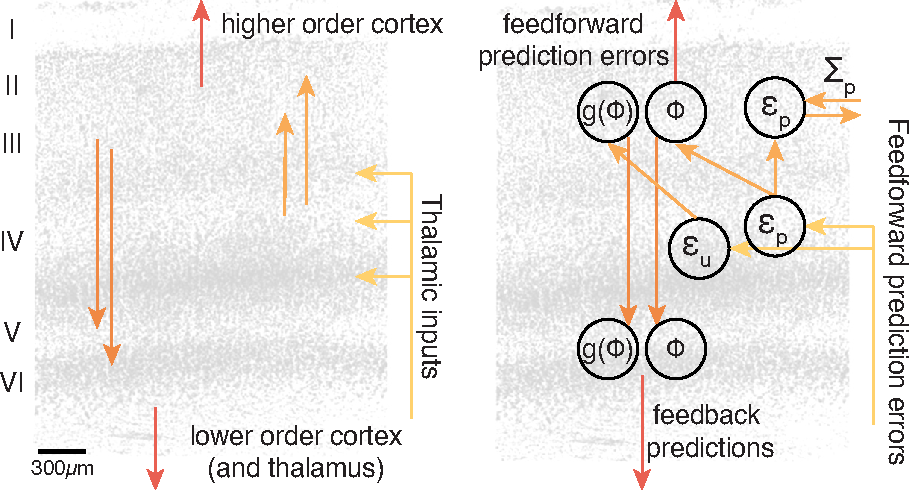
\includegraphics[width=1.\textwidth]{fig/chap2_fig_microcircuit.pdf}
\caption[Canonical microcircuit for predictive coding.]{Canonical microcircuit for predictive coding, with (left) Figure \ref{fig_chap2_vision_V1} for comparison and (right) graph adapted from Bastos~\cite{bastos2012canonical}.}
\label{fig_chap2_microcircuit}
\end{figure}

It now remains to review experimental proofs to back the existence of such predictive circuitry. In that sense, proofs of a canonical microcircuit are somewhat sparse, but there is growing consensus that a canonical microcircuit performing predictive operations does indeed account for experimental results. In this context, the study in chapter 4 provides further experimental support, by validating the idea of mapping input variance to supragranular layers, largely due to their extensive lateral connectivity~\cite{angelucci2002circuits,chavane2022revisiting, adesnik2010lateral}. There is also vast account of the fact that specific types of neurons in microcircuits - namely disinhibitory motifs~\cite{kuhlman2013disinhibitory, naka2016inhibitory} - are performing layer-specific computations~\cite{bugeon2022transcriptomic} that can support learning on-par with predictive coding algorithms~\cite{sacramento2018dendritic}.
Finally, there is also theoretical evidence that show that combining simple elements of neural origin can actually yield neural networks that compute prediction errors in an unsupervised manner~\cite{boerlin2013predictive, hertag2022prediction}.

Further, this model implies that predictions and prediction errors, operating mostly on two separate firing regimes, are reflected in the oscillatory domain (an experimental concept further explored in chapter 7). Based on that observation, there is a mounting evidence that suggest two bands of oscillations for superficial and deep layers of the cortex~\cite{bastos2015visual}. Such oscillatory evidences are numerous~\cite{nikolic2013gamma, schmiedt2014beta, engel2001dynamic, engel2010beta} to show that deep layers oscillate at a low frequency~\cite{bastos2020layer} (which is gated through the pulvinar~\cite{cortes2021corticothalamic}, as contributed in chapter 7) to prepare predictions and make way for the fast oscillations of sensory inputs in upper layers.

On a broader scale, numerous empirical evidences of predictive coding mechanisms at work in the brain have been accumulated, even prior to Friston's initial paper, which we will now explore to further support our approach.



\newpage 



\subsection{The in-vivo implementational level: Neurobiology}
The final part of this introduction to the implementational level involves transitioning from the notion that predictive coding can be used as a framework for this thesis, towards showing proof that there exists both predictive and variance-based computations in the brain.




\subsubsection{Neural evidences of predictive coding}
Having gathered the (sparse) supporting biological evidence for a canonical microcircuit, and having mapped this predictive microcircuit to certain functional activity at the circuit level, we now turn our attention towards assessing whether the brain indeed utilizes predictive coding at a global scale. A bias naturally stems here~\cite{shipp2016neural}, as we will try to explain many disparate phenomena with a single theory - when one perceives every problem as a nail, it becomes convenient to envision a normative theory based on a hammer~\cite{maslow1966psychology}. 

Essentially, as we expressed in Equation \ref{eq_df_derror_final}, predictive coding proposes that the brain increases computational efficiency by transmitting only prediction errors~\cite{friston2005theory}. As such, if a certain visual input does not generate a prediction error, it should not be transmitted, and thus the neural response for predicted stimuli should be weaker than for unpredicted stimuli. Therefore, the first argument that supports the existence of predictive coding in the brain is the experimental observation that repetition of stimuli elicit a diminution of the evoked neural activity. This is observable not just with the visual responses~\cite{summerfield2008neural, summerfield2011human}, but also in the auditory~\cite{garrido2007evoked, todorovic2011prior} and somatosensory cortices. 
Conversely, unexpected or surprising events should trigger an increase in said neural activity. This assertion is also verified within the visual pathways~\cite{pak2021impaired} where the violation of a repetitive pattern induces a significant surge in the firing rate. This effect is also noticeable at the psychophysical level, a neural event known mismatch negativity potential~\cite{alho1995cerebral, wacongne2012neuronal}, which is an entire sub-field on its own (see chapter 7). Further evidences can be found when violating the distribution of natural images~\cite{bair2003time,fiser2004small} (as described in the first section of the introduction), or under many conditions of predictability violation~\cite{kok2012attention, meyer2011statistical,murray2002shape}.

It's also worth noting that the large-scale hierarchical organization of the cortex, particularly the visual cortex~\cite{felleman1991distributed}, aligns well with the principles of predictive coding (Figure~\ref{fig_chap2_brainlevel_pc}). In this representation, the hierarchical organization of the brain emerges from the Bayesian inference process we developed earlier, which relies on a hierarchical conditional model~\cite{friston2006free}. This corresponds well with the layer-specific responses of the microcircuit and their respective feedforward versus feedback connections~\cite{markov2014anatomy}. On a larger scale, this constitutes a recurrent circuit that generalizes the formulation we introduced in Equation~\ref{eq_pc_matrix}: a stable functional model that seeks to minimize prediction errors while continuously updating a prediction-based model of the world.

\begin{figure}[h!tbp]
\vspace{0.5cm}
\centering
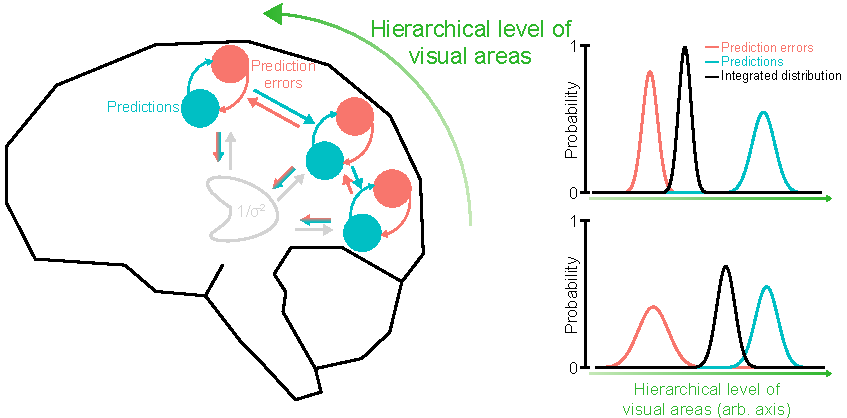
\includegraphics[width=1.\textwidth]{fig/chap2_fig_hierarchical_pc.pdf}
\caption[Hierarchical predictive coding in the brain]{Hierarchical predictive coding in the brain, (left) implemented as a globally and locally recurrent series of prediction errors and prediction integrations. (right) As in Figure \ref{fig_chap2_equi_proba_var}, the effect of the input variance on the predictive model.}
\label{fig_chap2_brainlevel_pc}
\end{figure}

Still on the anatomical side of the argument, the lateral connectivity intra~\gls{V1} merits further mention~\cite{thomson2003interlaminar,chavane2011lateral,katzel2011columnar}, as it provides the support for local competition of orientation-based predictions on the worldly states. This is usually characterized as an attentional mechanism~\cite{friston2012predictive,ainley2016bodily}, but we would contribute here that it takes effect far too rapidly~\cite{ladret2023cortical} for that to be the case. In this thesis, we interpret it as a local mechanism, as formulated by Friston in its original implementation of predictive coding~\cite{friston2005theory}.
Another implementation we will discuss in chapter 7 involves a globally parallelized (through the pulvinar) implementation of variance~\cite{kanai2015cerebral}, that allows the brain to determine which visual areas best explain the current environment. This is experimentally corroborated by the fact that pulvinar modulations essentially constitute contextual modulations~\cite{robinson1992pulvinar, casanova2001higher,de2020pulvinar} dynamically applying context to the content processed by the cortex~\cite{purushothaman2012gating}.

In addition to these findings, predictive coding has been shown to effectively model pathological conditions of the brain, an emerging field referred to as computational psychiatry~\cite{adams2013computational}.  While it's too premature to label this as evidence, the wide adoption~\cite{grenander1998computational} of this framework is a compelling argument supporting the idea of the brain functioning as a predictive system. In that framework, the idea that shifts in variance can move one closer or further from the prior, as demonstrated in Figure~\ref{fig_chap2_brainlevel_pc} (and in the Conclusion of this manuscript), provides a fitting description of disorders characterized by hypo-variant priors (such as autism~\cite{van2013predictive, van2014precise}) or hyper-variant priors (like schizophrenia~\cite{horga2014deficits}). This now paves the way for the end of this (lengthy) introduction, with a final (and not lengthy) section dedicated to the representation of variance in the predictive brain.

\newpage

\subsubsection{Neural representations of variance}
Having mapped predictive models onto some biological substrates, it is now time to explore whether there is empirical biological evidence supporting the representation of variance. Unfortunately, this field of investigation is not an expansive one, as reflected by the length of this section. What sparse evidence exist is however very promising, and in line with our respective contributions in chapters 3 to 8.

The seminal work in this field is a study by Orban et al.~\cite{orban2016neural}, which shows that local computations performed between orientation detectors can effectively process orientation variance, as that competition, through inhibition, increases the spike-to-spike variance of the neural activity. Thus, elegantly, the variance of an internal representation can be "signaled" by the variance of the activity supporting it. This aligns well with the psychophysical literature we introduced earlier~\cite{heeley1989width}, specifically the notion that competition among orientation detectors accounts for the psychophysical observations of human subjects. 

On the biological front, if we refrain from considering the superposition of two gratings as a distribution of orientation, as was historically done~\cite{geisler2001motion} (although some approximation hold~\cite{furmanski2000oblique,li2003oblique}), the whole idea of encoding orientation variance in \gls{V1} was actually pioneered by Goris et al.~\cite{goris2015origin}. They reported that heterogeneously tuned \gls{V1} populations help encode the orientation distributions found in natural images, and that this functional diversity could be accounted for by a linear-nonlinear (L-NL) model. While this could explain the diversity of tuning in the data we report in chapter 4, we will find that in terms of modeling, competition among orientation detectors within a predictive context remains the best descriptor~\cite{ladret2023cortical}. 

\begin{figure}[h!tbp]
\vspace{0.1cm}
\centering
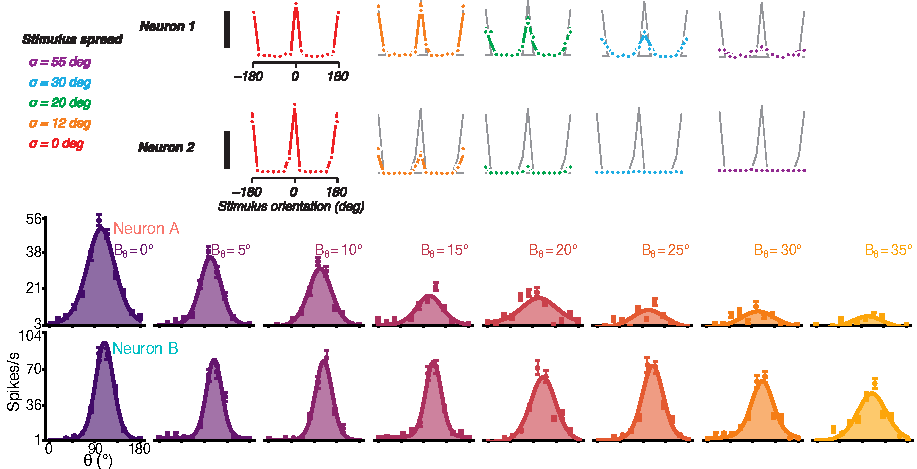
\includegraphics[width=1.\textwidth]{fig/chap2_fig_goris.pdf}
\caption[Active modulation of neurons by orientation variance.]{Modulation of tuning curves by orientation variance. (Top) Goris et al.~\cite{goris2015origin}. (Bottom) This thesis~\cite{ladret2023cortical}.}
\label{fig_chap2_neuralvariance}
\end{figure}

Considering the sparse nature of the relevant literature, referencing our own work from chapter 4 here feels necessary. Our study reaffirms the findings in the literature on anesthetized macaques~\cite{goris2015origin}, as we identified single-neuron variance modulations that underpin the decoding of orientation variance at the population level in \gls{V1}. This suggests that a shared neural mechanism may exist in both felines and primates, which isn't surprising given the crucial role of variance for the proper encoding of natural images in \gls{V1}~\cite{olshausen1996emergence}, a point we've emphasized repeatedly throughout this introduction. 

Our specific contribution here is connecting these findings to cortical layers, strengthening the idea that supragranular neurons with sharp tuning and slow dynamics~\cite{ringach1997dynamics,ringach2002orientation} facilitate the concurrent encoding of orientation and its variance. This links nicely with the concept of cortical microcircuit introduced earlier, as ten years prior to our article, it was proposed that supragranular activity should encode variance, a hypothesis for which we have provided formal experimental evidence in this thesis.

As far as biological evidences are concerned, there is consensus across studies that heterogeneity and local competition, i.e., intra-V1 activity, are sufficient to explain all observations. In fact, both neurobiological and computational evidence suggest that \gls{V1} doesn't need to enlist other cortical areas to process orientation variance, but that such process in other cortical areas might actually be part of synchronized global computations (more in chapter 7). 

For instance, the heterogeneous recurrent excitatory and inhibitory synaptic connectivity in \gls{V1}~\cite{jia2010dendritic, chen2011functional, iacaruso2017synaptic, scholl2017local} sustains resilient orientation tuning~\cite{monier2003orientation} that can account for the diversity of single neurons' resilience under different connectivity profiles, as explored in our computational model~\cite{ladret2023cortical}.
This is supported by the temporal scale of local recurrent connectivity, namely the slowly-conducted horizontal waves in an orientation map~\cite{chavane2011lateral}, which fits the view of variance processing as an iterative and accumulative computation implemented by local recurrent interactions between supragranular resilient neurons that are heavily connected through recurrent interactions with neighboring cortical columns~\cite{douglas1989canonical,ringach1997dynamics,ringach2002orientation, chavane2011lateral}. 

Despite the limited quantity of available evidence, the existing findings notably converge. Whether across species, research teams or functional encoding schemes, the overarching theme remains constant: there is an active encoding of variance in the primary visual cortex. Having established this, we can now proceed to explore the main section, beginning with the exploration of the structure of variance in natural images, which will then directly link to the findings in chapter 4.